\documentclass[preprint]{aastex}

% packages for figures
\usepackage{graphicx}
% packages for symbols
\usepackage{latexsym,amssymb,hyperref}
% AMS-LaTeX package for e.g. subequations
\usepackage{amsmath}


\usepackage[OT2,T1]{fontenc}


%=====================================================================
% FRONT MATTER
%=====================================================================

\slugcomment{Draft \today}

%=====================================================================
% BEGIN DOCUMENT
%=====================================================================

\newcommand{\klim}{\ensuremath{k_\mathrm{lim}}}
\newcommand{\kmax}{\ensuremath{k_\mathrm{max}}}
\newcommand{\kmin}{\ensuremath{k_\mathrm{min}}}
\newcommand{\rmd}{\ensuremath{\mathrm{d}}}
\newcommand{\beq}{\begin{equation}}
\newcommand{\eeq}{\end{equation}}
\newcommand{\mi}{{\rm i}}
\newcommand{\me}{{\rm e}}

\DeclareSymbolFont{cyrletters}{OT2}{wncyr}{m}{n}
\DeclareMathSymbol{\Sha}{\mathalpha}{cyrletters}{"58}

\begin{document}

\title{The GalSim lensing engine}

\begin{abstract}
This document describes the GalSim ``lensing engine'' for drawing
shears randomly according to a user-specified shear power spectrum.
It includes a brief description of the theory behind shear power
spectra, the connection between the usual continuous description of
the theory versus our representation in terms of the discrete Fourier
transform, and a validation of the outputs for several test cases.
\end{abstract}

\tableofcontents

\section{Introduction}

The lensing engine (in galsim/lensing.py) is the part of GalSim that
is supposed to draw shears randomly according to a user-specified
power spectrum.  In this document, we begin with a brief description
of the theory behind shear power spectra (\S\ref{sect:theory}), and then clarify the following
issues:
\begin{enumerate}
\item How does the discrete representation that we use (on a grid)
  relate to the standard formulation of the theory, which uses
  continuous representations?  (\S\ref{S:discrete})
\item Are our outputs consistent with expectations?
\begin{itemize}
\item How does it compare with another standard piece of software that
  generates shears using a different formalism? (\S\ref{S:comparison})
\item Is the normalization (expressed as a variance) correct? (\S\ref{S:testvar})
\item Does the variance behave appropriately when the grid size and
  spacing is changed? (\S\ref{S:testvar})
\item Does the full $P(k)$ of the shears that were generated agree
  with our expectations?  Does the result behave appropriately when
  the grid size and spacing is changed? (\S\ref{S:testpk})
\item Is the behavior appropriate when inputting only $E$ mode power,
  only $B$ mode power, and both $E$ and $B$ mode power? (\S\ref{S:testpk})
\end{itemize}
\item We should consider the impact of our current choice to force
  $P(k=0)=0$, which effectively says there is no cosmic variance. (\S\ref{S:pk0})
\end{enumerate}


\section{Theory}\label{sect:theory}

\subsection{Continuous representation}

The lensing engine requires a shear power spectrum, $P(k)$, and
assumes we are in the flat-sky limit.  Many standard references
regarding lensing power spectra work in terms of the spherical
harmonics $\ell$, with the power spectrum denoted $C_\ell$.  In the
flat-sky limit we can simply swap $\ell$ with $k$ and $C_\ell$ with
$P(k)$.  It is standard practice to plot a dimensionless quantity
$\Delta^2$ defined as
\beq
\Delta^2 = \frac{\ell(\ell+1) C_{\ell}}{2\pi}\equiv \frac{k^2 P(k)}{2\pi}.
\eeq

If we identify pairs of galaxies separated by an angle $\theta$ on the
sky, and compute their shears in a coordinate
system defined along the vector connecting them ($\gamma_+$) and at 45
degrees with respect to it ($\gamma_\times$), then we can estimate 
correlation functions of the $\gamma_+$ and $\gamma_\times$ values,
which we will call $\xi_{++}$ and $\xi_{\times\times}$.  Then the
standard cosmological correlation functions $\xi_{\pm}$ are defined as
\begin{align}
\xi_{\pm}(\theta) &=  \xi_{++}(\theta)\pm \xi_{\times \times}(\theta) \\
 &= \frac{1}{2\pi}\int_0^{\infty} k\,\rmd k P(k) J_{0/4}(k\theta)  \label{eq:xi}
\end{align}
where $J_{0/4}$ denotes the 0th and 4th Bessel function of the first
kind, as is appropriate for $\xi_+$ and $\xi_-$, respectively. 
Since correlation functions are dimensionless, we immediately see that
$P(k)$ has dimensions of angle$^2$.

The variance of the shear values for all of our galaxies is the zero-lag value of $\xi_+$, 
\beq\label{E:shearvar-basic}
\mathrm{Var}(\gamma) = \xi_{+}(\theta=0) = \langle g_1^2 + g_2^2\rangle.
\eeq
Combining Eqs.~\ref{eq:xi} and \ref{E:shearvar-basic}, we can write
the shear variance in terms of the power
spectrum
\beq\label{E:shearvar}
\mathrm{Var}(\gamma) = \frac{1}{2\pi}\int_0^{\infty} k\,\rmd k P(k),
\eeq
which essentially says the shear variance is the power integrated over
the allowed area in $k$ space.

\subsection{Representation on grids}

We will have to modify the above formalism to account for the fact
that all of our calculations use a discrete representation on a finite
grid.  This 
grid is defined by
\begin{align}
L &= \mbox{length of grid along one dimension (angular units)}\\
d &= \mbox{spacing between grid points (angular units)}\\
N &= \mbox{number of grid points along one dimension} = L/d.
\end{align}
Given this grid, the \kmin\ along one dimension is $2\pi/L$, so we can
think of this quantity as the grid spacing in Fourier space, i.e.,
$\kmin=\Delta k$.  This value of \kmin\ corresponds to a Fourier mode
that exactly fits inside of our square grid (in one dimension).  The
$k$ range, again in one dimension, is from $k_1=-\pi/d$ to $\pi/d$,
i.e., $|k_1|<\kmax=\pi/d$.  This corresponds to a mode that is sampled
exactly twice (the minimum possible) given our choice of grid
spacing.  For the two-dimensional grid, the maximum value of $|k|$ is
then $\sqrt{2}\pi/d$.

For a given grid point in
Fourier space, it is
somewhat a matter of taste as to whether it is considered to start at
that $k$ and extend to $k+\Delta k$, or whether it goes from $k-\Delta
k/2$ to $k+\Delta k/2$.  For the examples we will consider, the
difference between these two options is typically of order 1\%.  In
practice, the choice of convention just shifts the limits of
integration in the equations below by at most $\Delta k$.

In the context 
of power spectra for gridded quantities, instead of using
Eq.~\ref{E:shearvar} it is more useful to think in
terms of the 2D integral in Cartesian coordinates
\beq\label{E:alt-shearvar}
\mathrm{Var}(\gamma) = \frac{1}{(2\pi)^2} \int_{-\infty}^{\infty} \rmd k_1 \,\rmd k_2 \,
P(k_1, k_2).
\eeq
Note that this equation assumes that our grid is infinite and $P(k)$
is defined for all $k$.  With a limited $k$
range, and with the power spectrum forced to $P(0)=0$ (see \S\ref{S:pk0}
for more discussion of this), we can rewrite Eq.~\ref{E:alt-shearvar} as
\beq\label{E:alt-shearvar-limit}
\mathrm{Var}(\gamma) = \frac{4}{(2\pi)^2} \left[\int_{0}^{\kmax}\int_{0}^{\kmax} \rmd
k_1 \rmd k_2 P(k) - \int_{0}^{\kmin}\int_{0}^{\kmin} \rmd k_1 \rmd k_2
P(k)\right].
\eeq
Here the factor of $4$ compensates for the 
quadrants that are not represented explicitly (i.e., negative $k_1$
and/or $k_2$ values).

Another interesting point about gridded quantities is that it is not
clear that we 
can enforce/check behavior of Var($\gamma_1$) or Var($\gamma_2)$,
particularly if 
there is a lot of shear power at small $k$.  Probably we should 
 only expect normal behavior for Var($\gamma$), but it's still worth
 verifying this explicitly in Sec.~\ref{S:testvar}.

In the limit that our power spectrum drops to zero at
\kmax, and that there is not too much power in the range $0<k<\kmin$
relative to that in $\kmin<k<\kmax$, Eqs.~\ref{E:shearvar}, \ref{E:alt-shearvar}, and
\ref{E:alt-shearvar-limit} should all give the same answer.

The above equations just include $P(k)$, but in principle there can be
two such functions, $P_{E}$ and $P_B$.  These should simply be summed
in Eqs.~\ref{E:shearvar}, \ref{E:alt-shearvar}, and
\ref{E:alt-shearvar-limit}.

\section{Representing continuous fields using the Discrete Fourier Transform}\label{S:discrete}

This section includes is the formalism describing what the GalSim
lensing engine is actually doing when representing shear fields as
discrete fields defined on a finite grid, as opposed to the continuous
representation in \S\ref{sect:theory}.

\subsection{Conventions}

The definition of the correlation function in equation \eqref{eq:xi}
employs the \emph{angular frequency, non-unitary}\footnote{According
  to the paradigm described in
  http://en.wikipedia.org/wiki/Fourier\_transform\#Other\_conventions}
definition of the (1D) Fourier transform:
\begin{eqnarray}
\tilde{f}(k) & = & \int_{-\infty}^{\infty} f(x) \me^{-\mi k x}
\rmd x ~ ~ \equiv ~ \mathcal{F} \{ f(x) \} \label{eq:fwdft} ; \\
f(x) & = & \frac{1}{2 \pi} \int_{-\infty}^{\infty} \tilde{f}(k) \me^{\mi k x}
\rmd k ~ ~ \equiv ~ \mathcal{F}^{-1}\{ \tilde{f}(k) \} \label{eq:invft}, 
\end{eqnarray}
with the usual simple generalizations to two or more dimensions.

The standard results in Discrete Fourier Transform (DFT) and its halfway-house the Discrete Time Fourier Transform (DTFT) are all derived under the unitary (i.e.\ without asymmetric prefactors of $1/2\pi$) convention in the online literature, adding to the complexity of interpretation.  In the next section, we present some of the standard results of Fourier theory using the angular frequency, non-unitary convention above, since we will require them in Section \ref{sect:DFTPS}.

\subsection{Fourier transform properties}
It can be readily shown that if we define $g(x L) \equiv f(x)$, the following well-known identity holds
under our Fourier transform convention:
\begin{equation}
\mathcal{F}\{g(x L)\} = \frac{1}{L}
\tilde{g}\left(\frac{k}{L}\right). \label{eq:gmult}
\end{equation}
If we further define $s(h + x) \equiv g(x)$ then it is straightforward
to show that
\begin{equation}
\mathcal{F}\{ s(h + x) \} = \me^{\mi k h} \tilde{s}(k).  \label{eq:sadd}
\end{equation}
Here we begin to get divergent results between conventions: there is
an additional factor of $2\pi$ in the exponent when this property of
FTs is expressed using the normal frequency
convention.

The most important result for approximating continuous functions using
DFTs is the Poisson summation formula, which under our conventions may
be stated as
\begin{equation}
\sum_{n=-\infty}^{\infty} f(n) = \sum_{q=-\infty}^{\infty} \tilde{f}(2
\pi q)
\end{equation}
for integers $n$ and $q$.  This result can be derived by writing the
  expression for the inverse Fourier transform of $\tilde{f}(2 \pi
q)$ and considering the Fourier series expansion of the periodic Dirac comb
function
\begin{equation}
\Sha_L (x) = \sum_{n=-\infty}^{\infty} \delta(x - nL).
\end{equation}
It should be noted that in the normal frequency, unitary transform
convention form of the Poisson summation formula the $2\pi$ within $\tilde{f}(2 \pi
q)$ is absent.  Using equation \eqref{eq:gmult} we then find
\begin{equation}
\sum_{n=-\infty}^{\infty} f(n L) = \frac{1}{L}
\sum_{q=-\infty}^{\infty} \tilde{f} \left(\frac{2 \pi q}{L} \right),
\end{equation}
which can be modified further using equation \eqref{eq:sadd} to give
the most useful expression of the Poisson summation formula:
\begin{equation}
\sum_{n=-\infty}^{\infty} f(n L + x) = \frac{1}{L}
\sum_{q=-\infty}^{\infty} \tilde{f} \left(\frac{2 \pi  q}{L} \right)
\me^{\mi 2 \pi x q / L}.
\end{equation}
If we define $\Delta k \equiv k_{\rm min} = 2 \pi / L$ we can also write
this as
\begin{equation}
\sum_{n=-\infty}^{\infty} f\left(\frac{2\pi n}{\Delta k} + x \right) = 
\left(\frac{\Delta k}{2 \pi} \right)
\sum_{q=-\infty}^{\infty} \tilde{f} \left(q \Delta k \right)
\me^{\mi x \Delta k q }. \label{eq:poisson}
\end{equation}
These results give us most of what we need to understand DFTs with the
non-unitary Fourier transform convention commonly adopted for weak
lensing power spectra in the flat sky approximation.

\subsection{The Fourier transform of discrete samples of the power spectra}\label{sect:DFTPS}
In what follows we are going to derive results only for the $\xi_+$
correlation function of equation \eqref{eq:xi}.  This will not impact
the understanding of how $P(k)$ is approximated using DFTs, but allows
us to replace $\xi_{\pm}$ and $J_{0/4}(k \theta)$ in equation
\eqref{eq:xi} with the simpler $\xi_+$ and $J_0$, respectively.  We will just be aware subsquently that real ellipticity fields have two components, to be treated as described by equation \eqref{eq:xi}.

The inverse Fourier transform of $P(k)$ to give $\xi_+(\theta)$ may be written in Cartesian coordinates as
\begin{equation}
  \xi_{+}(\theta_1, \theta_2)  = \frac{1}{(2 \pi)^2} \int \! \! \!
  \int_{-\infty}^{\infty} P(k_1, k_2) ~ \me^{\mi (k_1 \theta_1 + k_2
  \theta_2)} \, \rmd k_1 \, \rmd k_2. \label{eq:xip}
\end{equation}
The relation between this and equation \eqref{eq:xi} makes use of Bessel's first
integral:
\begin{equation}
J_n(z) = \frac{\mi^{-n}}{\pi} \int_0^{\pi} \me^{\mi z \cos{\theta}}
\cos{(n \theta)} \, \rmd \theta.
\end{equation}

What happens if we only have finite samples of $P(k_1, k_2)$?  To
answer that, let us define the following function:
\begin{equation}
P_{\Delta k} [q, p] \equiv (\Delta k)^2 P(q \Delta k, p \Delta k).
\end{equation}
As here, we will use square brackets to denote functions with
discrete, integer input variables.  We will also use indices $n, m$ in
real space summations and $q, p$ in Fourier space ($i,j$ are awkward
due to the common notations for $\sqrt{-1}$).  Let us also define the 2D Dirac
comb function in Fourier space
\begin{equation}
\Sha^2_{\Delta k} (k_1, k_2) = \sum_{q = -\infty}^{\infty} \delta(k_1
- q \Delta k) \sum_{p = -\infty}^{\infty} \delta(k_2
- p \Delta k).
\end{equation}
It can then be shown that
\begin{eqnarray}
~ &~& \mathcal{F}^{-1} \left\{\sum_{q,p = -\infty}^{\infty} \delta(k_1
- q \Delta k) \, \delta(k_2
- p \Delta k) \, P_{\Delta k} [q, p] \right\} \nonumber \\
~ & = & \mathcal{F}^{-1} \left\{ P(k_1, k_2) \cdot  (\Delta
  k)^2 \Sha^2_{\Delta k} (k_1,
  k_2) \right\}  \nonumber  \\
 & = & \mathcal{F}^{-1} \left\{ P(k_1, k_2) \right\} * \mathcal{F}^{-1} \left\{  (\Delta
  k)^2 \Sha^2_{\Delta k} (k_1, k_2) \right\} \nonumber \\
 & = & \xi_+(\theta_1, \theta_2 )  * \left\{ \sum_{n = -\infty}^{\infty} \delta\left(\theta_1
- \frac{2 \pi n}{\Delta k} \right) \sum_{m = -\infty}^{\infty}
\delta\left( \theta_2
- \frac{2 \pi m}{\Delta k} \right)  \right\} \nonumber \\
& = & \sum_{n,m=-\infty}^{\infty} \xi_+\left(\theta_1
- \frac{2 \pi n}{\Delta k},  \theta_2
- \frac{2 \pi m}{\Delta k} \right) \label{eq:xisum}
\end{eqnarray}
Here we have again made use of the Fourier series expression for the
Dirac comb function, and employed the convolution theorem (convolution
denoted with $*$).  We note that the final expression \eqref{eq:xisum}
is still continuous, but describes an infinite, periodic summation (of period $L = 2 \pi
/ \Delta k$) of copies of the correlation function $\xi_+$.  For sufficiently small
$\Delta k$, these copies may be well-enough spaced in the real domain to
learn much about $\xi_+(\theta_1, \theta_2)$ in the non-overlapping
regions.

We therefore define this function as
\begin{equation}
\xi_{\frac{2\pi}{\Delta k}}(\theta_1, \theta_2) \equiv \sum_{n = -\infty}^{\infty} \xi_+\left(\theta_1
- \frac{2 \pi n}{\Delta k},  \theta_2
- \frac{2 \pi m}{\Delta k} \right).
\end{equation}
Using the expression of the Poisson summation formula in equation
\eqref{eq:poisson}, we can also write the result
\begin{equation}
\xi_{\frac{2\pi}{\Delta k}}(\theta_1, \theta_2) =
\sum_{q,p=-\infty}^{\infty} \left( \frac{\Delta k}{2 \pi} \right)^2 P(q \Delta k, p \Delta k) \me^{\mi \Delta
  k (\theta_1 q + \theta_2 p)} = \frac{1}{( 2 \pi)^2}
\sum_{q,p=-\infty}^{\infty} P_{\Delta k} [q, p] \me^{\mi \Delta
  k (\theta_1 q + \theta_2 p)} \label{eq:dtft} 
\end{equation}
(which, like the Poisson summation formula, can also be shown using
equation \ref{eq:xisum} and substituting the Fourier series expression
for $\Sha^2_{\Delta k}$).  This is the expression for the inverse of
what is known as the Discrete Time Fourier Transform (DTFT), although
this result is normally derived using unitary conventions for the
transform pair.  Note that the terms $P_{\Delta k}[q, p]$ are
dimensionless, being composed of $(\Delta k)^2 = (2 \pi / L)^2$
multiplied by the samples $P(q \Delta k, p \Delta k)$ of the power
$P(k_1, k_2)$ (with dimensions of angle$^2$).

One intuitive way of looking at the approximation of equation \eqref{eq:xip} for the case of discretely
sampled $P(k_1, k_2)$ is that the terms in the discrete sum should be
considered as \emph{impulses} of area $(\Delta k)^2$ and height $P(q \Delta k, p \Delta k)$.

\subsection{The Fourier transform of discrete, finite samples of the power spectra}
The expression in equation \eqref{eq:dtft} is periodic with period $2
\pi / \Delta k = L$.  All of the information it contains about
$\xi_+ (\theta_1, \theta_2)$ is therefore also contained in one period
of the function only.  For approximating this information discretely, as desired in
numerical analysis, we can imagine taking $N$ equally spaced samples of
the function in equation \eqref{eq:dtft} along a single period $L$ in each
dimension (leading to $N^2$ samples total since we are working in 2D).
These samples are therefore separated by $\Delta \theta = 2 \pi /
\Delta k N = d$ in real space, and we define the sampled
function itself as
\begin{equation}
\xi_{\Delta \theta}[n, m] \equiv \xi_{\frac{2 \pi}{\Delta
    k}} \left( n \Delta \theta, m \Delta \theta \right) = \frac{1}{( 2 \pi)^2}
\sum_{q,p=-\infty}^{\infty} P_{\Delta k} [q, p] \me^{\mi 2 \pi (qn +
  pm) / N},
\end{equation}
for the integer indices $n, m = 0, 1, \ldots, N-1$, by substitution into equation
\eqref{eq:dtft}.  Using the periodicity of the exponential term in the
expression above, this may be written as
\begin{equation}
\xi_{\Delta \theta}[n, m] = \frac{1}{( 2 \pi)^2}
\sum_{q,p=0}^{N-1} P_N [q, p] \me^{\mi 2 \pi (qn +
  pm) / N}
\end{equation}
where we have defined
\begin{equation}
P_N[q, p] \equiv \sum_{i,j=-\infty}^{\infty}  P_{\Delta k} [q - i N, p
- j N] .
\end{equation}
Needless to say, in order to be able to calculate the values of
$P_N[q, p]$ in practice we must also truncate the 
$P_{\Delta k}$ sequence to be finite in length.  A \emph{very} common
choice is to use the same number $N$ of samples in both real and
Fourier space: this is also efficient, as it allows the direct use of
the Fast Fourier Transform algorithm.  We will say a little more about
this below.

Choosing to use only $N$
samples from $P_{\Delta k}$ then gives us a somewhat more
familiar expression for the inverse Discrete Fourier Transform (DFT),
written here for the non-unitary Fourier transform convention:
\begin{equation}
\xi_{\Delta \theta}[n, m] = \frac{1}{( 2 \pi)^2}
\sum_{q,p=0}^{N-1} P_{\Delta k} [q, p] \me^{\mi 2 \pi (qn +
  pm) / N}. \label{eq:dft}
\end{equation}
The overwhelmingly more common definition of the inverse DFT, and that adopted by
NumPy, instead reads as:
\begin{equation}
f[n, m] = \texttt{numpy.fft.ifft2}\left(\tilde{f}[p, q]\right) \equiv \frac{1}{N^2}
\sum_{q,p=0}^{N-1} \tilde{f}[q, p] \me^{\mi 2 \pi (qn +
  pm) / N} ,~~~~ (\textrm{NumPy convention}) \label{eq:dftnumpy}
\end{equation}
where the factor of $1/N^2$ is a convention commonly found in DFT
implementations, and ensures
that the DFT followed by the inverse DFT yields the original, input array.

We must use the convention of equation \eqref{eq:dftnumpy} for
performing the calculation within the code, and so this means that we
must attempt to account for the factors of $2 \pi$, $N$ and $\Delta
k$ ourselves.  Let us begin with the user specifying the
key dimensions of the problem $L$ and $d = \Delta \theta$ at the
outset, as assumed in Section \ref{sect:theory}, sensibly chosen (of
course) so that $N=L/\Delta \theta$ is an integer.  These choices also
set $\Delta k = 2 \pi / L$.  Beginning with equation
\eqref{eq:dft}, we may re-express the convenient $P_{\Delta k}[q, p]$ as
samples of the dimensional $P(k_1, k_2)$ once again:
\begin{eqnarray}
\xi_{\Delta \theta}[n, m] & = & \frac{1}{( 2 \pi)^2}
\sum_{q,p=0}^{N-1} P_{\Delta k} [q, p] \me^{\mi 2 \pi (qn +
  pm) / N}  \\ & = & \frac{1}{(2 \pi)^2} \times \frac{(2 \pi)^2}{L^2}
 \sum_{q,p=0}^{N-1} P(q \Delta k, p \Delta k) \me^{\mi 2 \pi (qn +
  pm) / N} \\
& = & \frac{1}{L^2} \sum_{q,p=0}^{N-1} P(q \Delta k, p \Delta k) \me^{\mi 2 \pi (qn +
  pm) / N} \\
& = & \texttt{numpy.fft.ifft2}\left[P(q \Delta
  k, q \Delta k) / (\Delta \theta)^2\right].
\end{eqnarray}
This equation explains why we require a division of the amplitudes by
$d=\Delta\theta$ in the lensing engine.  Dimensional analysis tells us
that we require a division by something with dimensions of angle, but
this equation is justification for exactly what angle is used.

Finally, we said we would say little more about the implications of
the choice to use $N$ as the
number of samples in \emph{both} real and Fourier space, the final step in
arriving at equation \eqref{eq:dft}.  This choice ensures the
close interrelation of $N$, $L$ and the grid spacings $\Delta \theta$,
$\Delta k$.  The use of discrete, periodic sampling to represent
continuous, non-periodic functions is only an approximation, and
one that depends heavily on good choices of these interrelated sampling
parameters.

The two effects that must be minimized for a good approximation are of course
aliasing and unwanted
`overlapping' of functions in either real or Fourier space due to the
sampled, periodic
representation inherent in the DFT.  Adequately sampling our functions, and zero-padding
them where possible to artificially extend $L$, are the primary
strategies for making the DFT and its inverse a good approximation to
the Fourier transforms of equations \eqref{eq:fwdft} and
\eqref{eq:invft}.


\section{Comparison software}\label{S:comparison}

We will compare the outputs from GalSim against those from a completely independent piece of software,
Chris Hirata's spherical harmonic transform code which is described in
multiple papers (for example,
\href{http://adsabs.harvard.edu/abs/2004PhRvD..70j3501H}{Hirata
  et~al. 2004}).  This does not use the flat-sky
approach, but that should not make too much difference even
for our $L=10$ deg.  It is something to bear in mind if we start
looking for agreement at a few \% level on the largest $\theta$ or
smallest $k$.  That software wants $C_\ell(\ell)$ as its inputs.

\section{Tests of variances}\label{S:testvar}

We begin with tests of the shear variances from GalSim and the SHT
code.  The theoretical 
description for the variances was outlined in \S\ref{sect:theory}.

\subsection{General considerations}

As discussed in \S\ref{sect:theory}, most of our tests of the variance
will focus on the sum of the components, rather than the variance of
individual components.  Also, for our grid to properly represent the
theoretical power spectrum (and for the equations in
\S\ref{sect:theory} to be valid), we need to be well-sampled in $k$
space, so we should not use functions that do unreasonable things like
$P(k)\propto k^{-2}$.

Since we will want to check that the results behave properly when the
grid changes, we will do all tests in this section with three
different grids:
\begin{enumerate}
\item A standard GREAT10 grid, which has $L=10$ degrees and $N=100$,
  so $d=0.1$ degree$=360$ arcsec.
\item A grid with $L=5$ degrees and $N=50$, thus preserving $d$ and
  \kmax, while increasing \kmin\ (the Fourier-space grid spacing) by a
  factor of 2.
\item A grid with $L=10$ degrees and $N=50$, thus doubling $d$ and
  halving \kmax, while preserving the Fourier-space grid spacing
  (\kmin) compared to the original case.
\end{enumerate}

\subsection{Variance for Gaussian $P(k)$}

Our first test case is a Gaussian $P(k)$, i.e., $P(k) =
P_0 e^{-\sigma^2 k^2 / 2}$.  Here both $P_0$ and $\sigma^2$ both
have dimensions of angle$^2$.  By Eq.~\ref{E:alt-shearvar-limit}, this
means that we expect
\begin{align}
\mathrm{Var}(\gamma) &= \frac{4P_0}{(2\pi)^2} \left[\left(\int_{0}^{\kmax} 
e^{-\sigma^2 k^2/2} \,\rmd k\right)^2 - \left(\int_{0}^{\kmin} 
e^{-\sigma^2 k^2/2} \,\rmd k\right)^2\right] \\
 &= \frac{P_0}{2\pi\sigma^2}\left[ \left(\mathrm{Erf}(\kmax\sigma/\sqrt{2})\right)^2 - \left(\mathrm{Erf}(\kmin\sigma/\sqrt{2})\right)^2\right].\label{E:vargauss}
\end{align}

For each of the grids, we define the Gaussian $\sigma$ such that there
is essentially no power left at our \kmax: $\sigma\kmax=2.5$, or
$\sigma=286.5$ arcsec for the first two grids and $\sigma=573$ arcsec
for the last grid.  Given how large $\sigma\kmax$ is, in all cases,
$\mathrm{Erf}(\kmax\sigma/\sqrt{2})=0.988$.  The resulting values of
$\sigma\kmin$ for the three grids are $0.05$, $0.1$, and $0.05$, or
$\mathrm{Erf}(\kmin\sigma/\sqrt{2})=0.04$, $0.08$, and $0.04$ (since
these are squared in the above expression, they don't end up mattering
much).  With
$P_0=1$ arcsec$^2$, the predicted variances for the three grids are
$1.89\times 10^{-6}$, $1.88\times 10^{-6}$, and $4.72\times 10^{-7}$.

The code to do this once is:
\begin{verbatim}
import galsim
import numpy as np
test_ps = galsim.PowerSpectrum(lambda k : np.exp(-0.5*((286.5*k)**2)))
g1, g2 = test_ps.buildGriddedShears(grid_spacing=360., ngrid=100)
print np.var(g1), np.var(g2), np.var(g1)+np.var(g2)
g1, g2 = test_ps.buildGriddedShears(grid_spacing=360., ngrid=50)
print np.var(g1), np.var(g2), np.var(g1)+np.var(g2)
test_ps = galsim.PowerSpectrum(lambda k : np.exp(-0.5*((573.0*k)**2)))
g1, g2 = test_ps.buildGriddedShears(grid_spacing=720., ngrid=50)
print np.var(g1), np.var(g2), np.var(g1)+np.var(g2)
\end{verbatim}
We actually do this 1000 times to beat down the noise in the resulting
variances.

The results are $1.87\times 10^{-6}$, $1.85\times 10^{-6}$, and
$4.63\times 10^{-7}$ in the last case.  So we have the approximately
correct amplitude and scaling with the grid spacing and grid size, and
the results are 1\%, 1.5\%, and 2\% smaller than the predictions.

We also check what happens if we make all the grids larger by a factor
of 4 (in $N$, i.e., decrease \kmin\ by a factor of 4 while maintaining
\kmax).  In this case, the variances increase by 1-2\%, whereas the 
predictions  based on Eq.~\ref{E:vargauss} only increase by 0.1\%.
Thus, the results with grids that are a factor of two larger are
completely in accordance with the predictions, and the percent-level deviations for the
original grids can be explained by finite-gridding effects.

The variance is fairly evenly divided between components, but the
variance in $\gamma_2$ tends to be larger than the variance of
$\gamma_1$ by 3--4\%.  This is
likely because the $P(k)$ emphasizes large scales, where the grid
genuinely looks different along the diagonals as it does along the
coordinate axes.  It's a feature of using grids to represent shears
drawn randomly from a power spectrum with finite $P_E$ but with
$P_B=0$, not a bug. If we set $P_B=P_E$ (unlike in the above example 
where $P_B=0$) then this difference between the variances of
$\gamma_1$ and $\gamma_2$ vanishes.

\subsection{Variance for flat $P(k)$}

A flat $P(k)$ has a worrisome amount of power at large $k$, so we use
a modified version of it: We use $P(k)=P_0$ for $k\le$\klim, where
$\klim<\kmax$ for all the grids; and we set $P(k>\klim)=0$. Using
Eq.~\ref{E:alt-shearvar-limit}, we expect
\begin{align}
\mathrm{Var}(\gamma) &= \frac{4P_0}{(2\pi)^2}
\left[\frac{1}{4}\int_{0}^{\klim} 2\pi k\,\rmd k - \kmin^2\right] \\
 &= \frac{P_0}{\pi^2} \left(\frac{\pi}{4} \klim^2 - \kmin^2\right).
\end{align}

For the set of grids from the previous test, \kmin\ is
$0.000175$, $0.00035$, and $0.000175$ arcsec$^{-1}$.  We will set $\klim=10\kmin$,
so we can write
\beq
\mathrm{Var}(\gamma) = \frac{(25\pi-1) P_0 \kmin^2}{\pi^2}.
\eeq
With $P_0=1$, we expect
shear variances that are $2.4\times 10^{-7}$, $9.6\times 10^{-7}$,
and $2.4\times 10^{-7}$.

The code is
\begin{verbatim}
import galsim
import numpy as np
def pfunc1(k):
    parr = np.zeros_like(k)
    parr[k<=0.00175] = 1.
    return parr
def pfunc2(k):
    parr = np.zeros_like(k)
    parr[k<=0.0035] = 1.
    return parr
test_ps1 = galsim.PowerSpectrum(pfunc1)
test_ps2 = galsim.PowerSpectrum(pfunc2)
g1, g2 = test_ps1.buildGriddedShears(grid_spacing=360., ngrid=100)
print np.var(g1), np.var(g2), np.var(g1)+np.var(g2)
g1, g2 = test_ps2.buildGriddedShears(grid_spacing=360., ngrid=50)
print np.var(g1), np.var(g2), np.var(g1)+np.var(g2)
g1, g2 = test_ps1.buildGriddedShears(grid_spacing=720., ngrid=50)
print np.var(g1), np.var(g2), np.var(g1)+np.var(g2)
\end{verbatim}

Since the variances are noisy, we averaged the results over 10000
realizations\footnote{This takes about 1 minute to run on a single
  CPU.}, and found $2.36\times 10^{-7}$, $9.45\times 10^{-7}$, and
$2.36\times 10^{-7}$.  These are all $\sim 2$\% below my naive calculation.
Since the overall behavior is correct when we change the grid size and
spacing, it seems possible that this small discrepancy comes from some
finite-gridding effect.

If we redo the above test but double the values of `ngrid', thus
halving the step size of the grid in Fourier space, then the variances
increase slightly\footnote{This change is statistically significant given
the number of realizations.} to $2.4\times 10^{-7}$, $9.6\times 10^{-7}$, and
$2.4\times 10^{-7}$, so they are now completely consistent with the
predictions from before.  In principle the predictions also have to
change, since now we have $\klim=40\kmin$ and the \kmin\ decreases by
a factor of 4, but the predictions only increased by 1\% whereas the
results increased by 2\%.  This result supports the claim that finite-gridding
effects might be responsible for the slightly low variances, rather
than anything more problematic (i.e., a true bug).  Finite gridding
effects can be accounted for by including them in the
predictions before comparing with results.

\section{Test of full $P(k)$}\label{S:testpk}

We use a WMAP7 LCDM prediction for the cosmic shear signal for a
sample with $z_\mathrm{med}\sim 0.55$ as an input to both
the SHT code and ours.  Given the range of $\ell$ for which it is
defined, $2<\ell<2000$, we cannot use our standard grid, which 
has $\kmax=\sqrt{2}\times 1800=2546$ radians$^{-1}$.  So, for this test we use a grid with
$L=10$ degrees (as before), but $N=50$ (i.e., $d$ gets doubled), which
means a two-dimensional $\kmax=1273$ radians$^{-1}$.

Using the SHT code (\S\ref{S:comparison}), we made gridded shears for
$P_E=P(k)$ and $P_B=0$; $P_B=P(k)$ and $P_E=0$; and $P_E=P_B=P(k)$ (5
realizations of each).  For GalSim, since it is much faster, we
averaged over several hundred realizations.  It is crucial to inform
GalSim that the inputs have units of radians.

The python script test\_pk.py in devel/external/test\_gridshear/ does the following:
\begin{enumerate}
\item Generates shears according to this PS using GalSim.
\item Runs the GREAT10 power spectrum code on both (must flip sign of
  one shear component before doing so), and averages it over several
  noise realizations.
\end{enumerate}

The python script test\_pk\_sht.py in that directory does the following:
\begin{enumerate}
\item Manipulate outputs of the SHT code to be consistent with
  expectations (including one sign flip for e1).
\item Runs the GREAT10 power spectrum code on it.
\end{enumerate}

Finally, plot\_pk\_test.py in that directory plots the original and
simulated $P(k)$ based on these files.  The results for the three
cases (input $P_E$, input $P_B$, and input $P_E=P_B$) are in
Figures~\ref{F:pe}, \ref{F:pb}, \ref{F:peb}.

\begin{figure}
\begin{center}
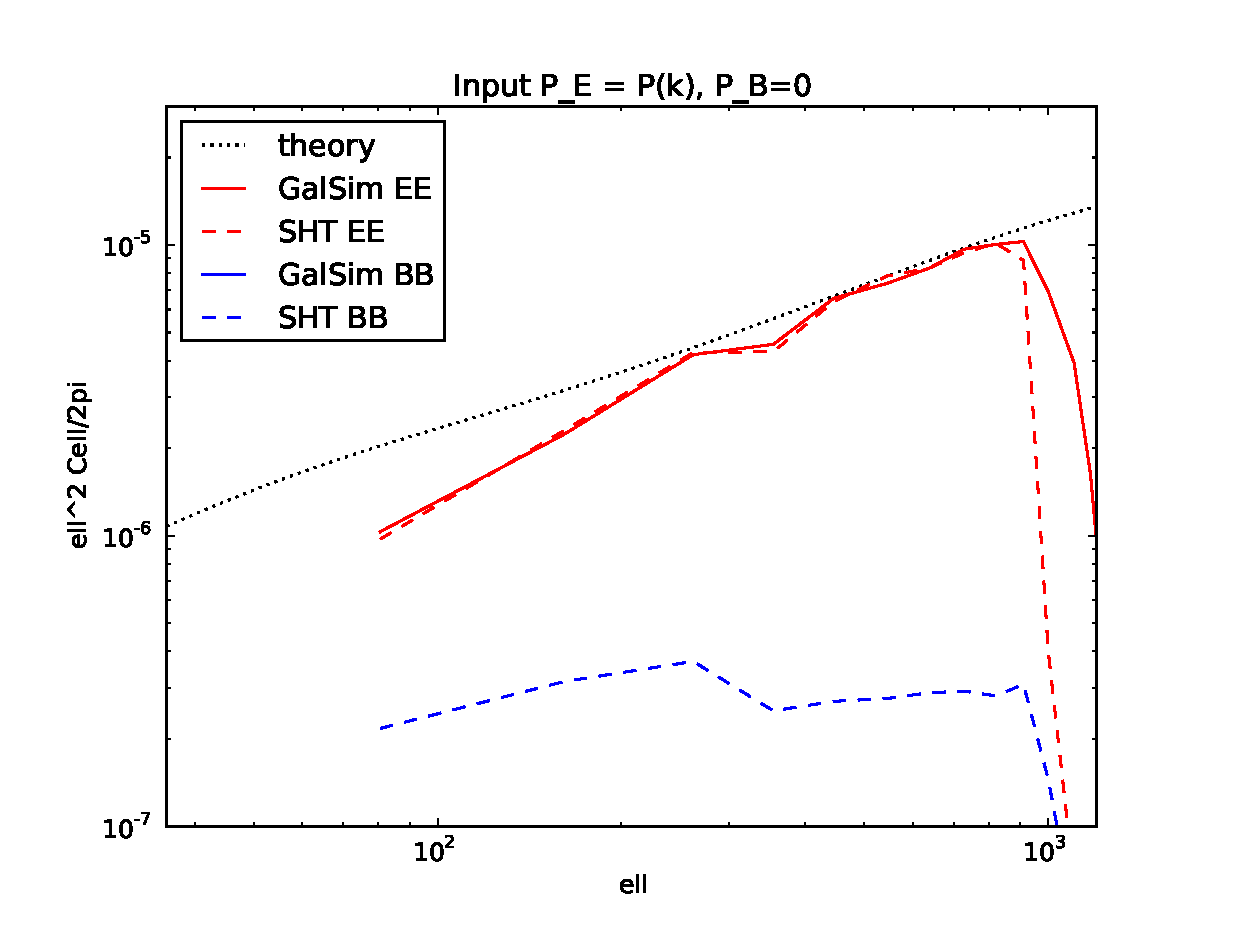
\includegraphics[width=3in]{../external/test_gridshear/output/compare_input_pe.eps}
\caption{Output shear power spectra (plotted as the dimensionless
  $\Delta^2$) for the grids described in Sec.~\ref{S:testpk}, where
  the input $P_E$ is a realistic cosmological one (shown as the `theory' line on
  the plot) and the input $P_B=0$. The results for GalSim and the
  comparison SHT code are both plotted.\label{F:pe}}
\end{center}
\end{figure}

\begin{figure}
\begin{center}
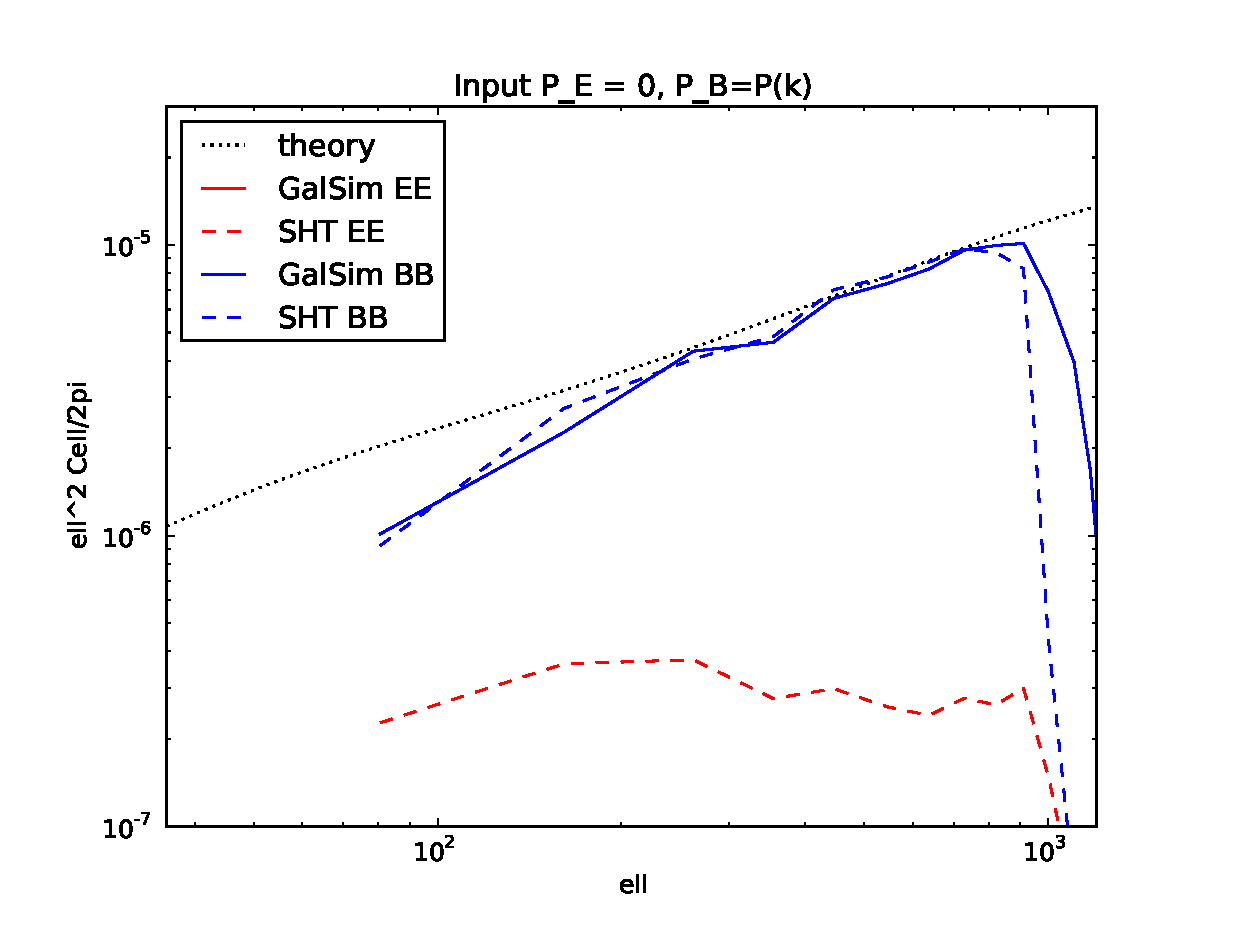
\includegraphics[width=3in]{../external/test_gridshear/output/compare_input_pb.eps}
\caption{Output shear power spectra (plotted as the dimensionless
  $\Delta^2$) for the grids described in Sec.~\ref{S:testpk}, where
  the input $P_B$ is a theoretical one and the input $P_E=0$. The results for GalSim and the
  comparison SHT code are both plotted.\label{F:pb}}
\end{center}
\end{figure}

\begin{figure}
\begin{center}
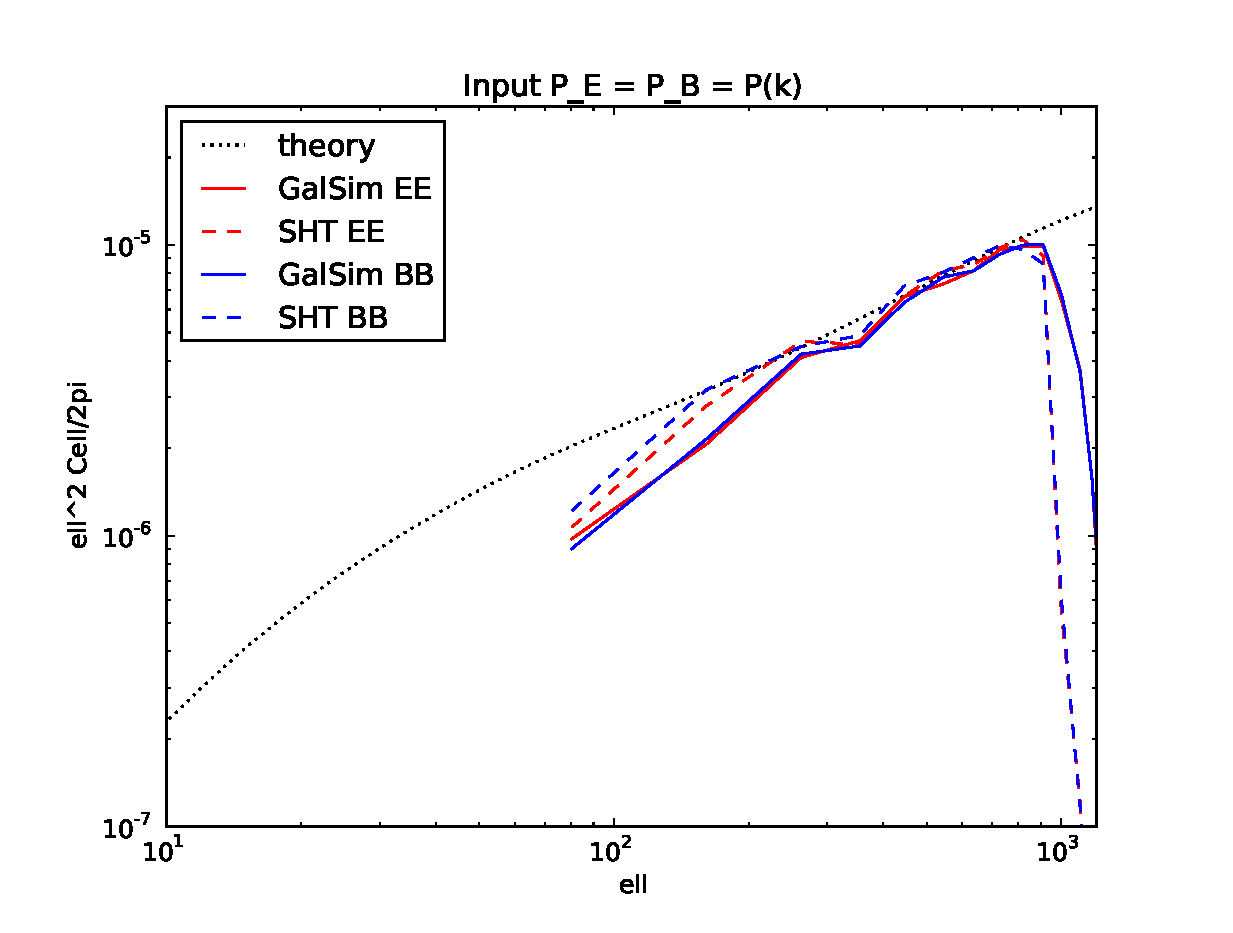
\includegraphics[width=3in]{../external/test_gridshear/output/compare_input_peb.eps}
\caption{Output shear power spectra (plotted as the dimensionless
  $\Delta^2$) for the grids described in Sec.~\ref{S:testpk}, where
  the input $P_E=P_B$ is shown as the `theory' line. The results for GalSim and the
  comparison SHT code are both plotted.\label{F:peb}}
\end{center}
\end{figure}

We can conclude several things from these figures:
\begin{itemize}
\item The SHT code gives roughly a consistent shear power spectrum compared
  to our inputs (modulo possible slight differences in scaling that
  may not be worth investigating until our own PS estimation code is ready),
  though there are signs of $E$ vs. $B$ leakage in the case where one
  or the other is zero.
\item GalSim: we don't see $E$ vs. $B$ leakage at any significant
  level.  The amplitudes and scaling of our output power spectra with
  $\ell$ are approximately correct.
\item The amplitude for the GalSim power spectra is slightly below that
  for the SHT code.  It is worth investigating whether this is some
  finite-gridding effect on our part.
\item While the big-picture results seem good, there are some finer
  details that require investigation, in particular the fact that both
  codes seem to give steeper $P(k)$ than the theory.  Given how these
  tests were done, it could have to do with the $k$-space binning in
  the power spectrum estimator, the sizes of the bins, etc. rather
  than some issue with GalSim.
  This is particularly true given that the SHT code was well-validated
  and exhibits nearly the same slope as the GalSim outputs.
\end{itemize}

To address the last point, the simplest possible test is simply to
change the $\ell$ binning in the PS estimation code.  This will let us
check whether we are encountering some finite-binning effects in the
PS estimation.  The original calculations had 20 $\ell$ bins; the new
one uses 50 within the same $\ell$ range.  To beat down the noise, we
used 400 realizations of the shears from GalSim, instead of 20 as
before.  The result is shown in Fig.~\ref{F:pe-fine}.  It is clear
that the results are, as compared to Fig.~\ref{F:pe}, closer to the
theory.  In particular, the amplitude {\em and} slope are both close
to theory for $\ell>100$.  Note that the jitter in that curve does not
go away if we use more realizations.  This could have to do with the
exact locations of the annular $\ell$ bins in the PS estimation code,
as compared to the finite set of $\ell$ modes that are probed by our
grid.

Since the log plot makes it hard to see how large differences between
theory and the GalSim results are, Fig.~\ref{F:pe-fine-ratio} shows
the ratio between the GalSim outputs and the theory.  For $\ell<100$,
the GalSim results are too low by $\sim 20$\%.  For $\ell>100$, the
GalSim outputs seems to give power spectra that are 5\% too low, which
is suspiciously similar to the results of the variance tests.  This
finding suggests that users {\em must} account for the effects of
finite $\ell$-binning on the theoretical power spectrum when
generating the shears, unless they
can choose sufficiently fine $\ell$ bins to minimize
this problem.  In support of this claim that finite gridding is
responsible, we found that with a grid that is doubled in size (and
hence a Fourier-space grid that is twice as finely spaced), the ratio
of observed to expected power spectrum is closer to 1 (but still 3\%
too low).

In detail, finite-gridding effects can arise because our gridded
approach amounts to estimating the power at specific $k_1$ and $k_2$
values (or rather in $k_1$ and $k_2$ bins of width $\Delta k$).  When
the PS estimator gets the power using the DFT approach, it's
essentially calculating these as $P(k=\sqrt{k_1^2 +k_2^2})$ which are,
again, defined at a set of specific values.  However, we then tell the
PS estimator ``tell me the power in some set of bins in $\log{k}$'', the
edges of which are not aligned in any particular way with respect to
our actual $k$ values at which we have estimated the power using the DFT
approach.  The PS estimator gets the power in each of our logarithmic
bins via summation over the $P(k)$ for all $k$ values that happen to fall
into that logarithmic bin.  This means there is some interplay between
the grid geometry (determining the $k$ values for which we'll have $P(k)$)
and the choice of log bins, which could result in jitter depending on
how the two relate.
\begin{figure}
\begin{center}
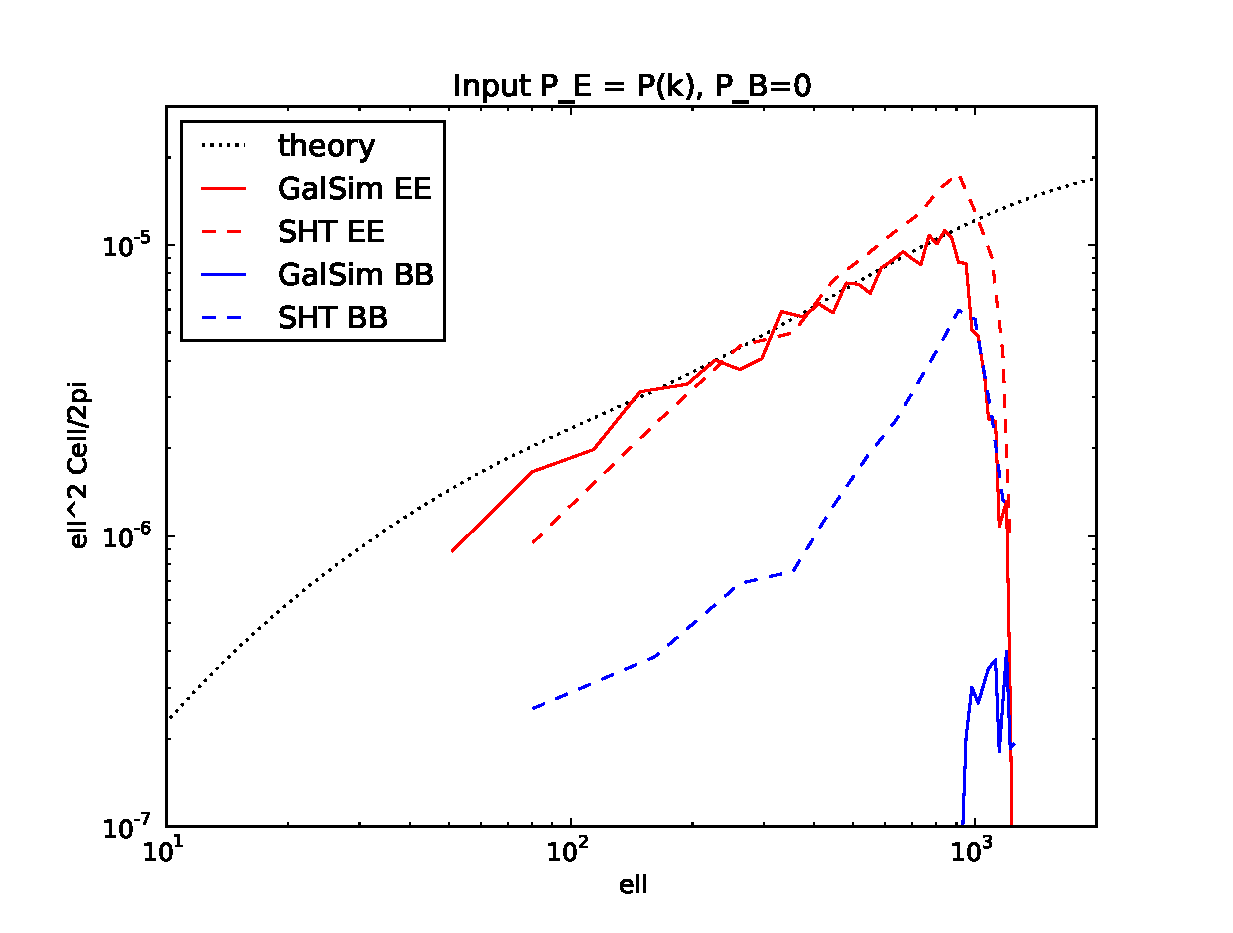
\includegraphics[width=3in]{../external/test_gridshear/output/compare_input_pe.fine.eps}
\caption{Output shear power spectra (plotted as the dimensionless
  $\Delta^2$) for the grids described in Sec.~\ref{S:testpk}, where
  the input $P_E$ is a realistic cosmological one (shown as the `theory' line on
  the plot) and the input $P_B=0$. The results for GalSim and the
  comparison SHT code are both plotted, but for GalSim we used 50
  $\ell$ bins in the PS estimation, rather than 20 as in Fig.~\ref{F:pe}.\label{F:pe-fine}}
\end{center}
\end{figure}
\begin{figure}
\begin{center}
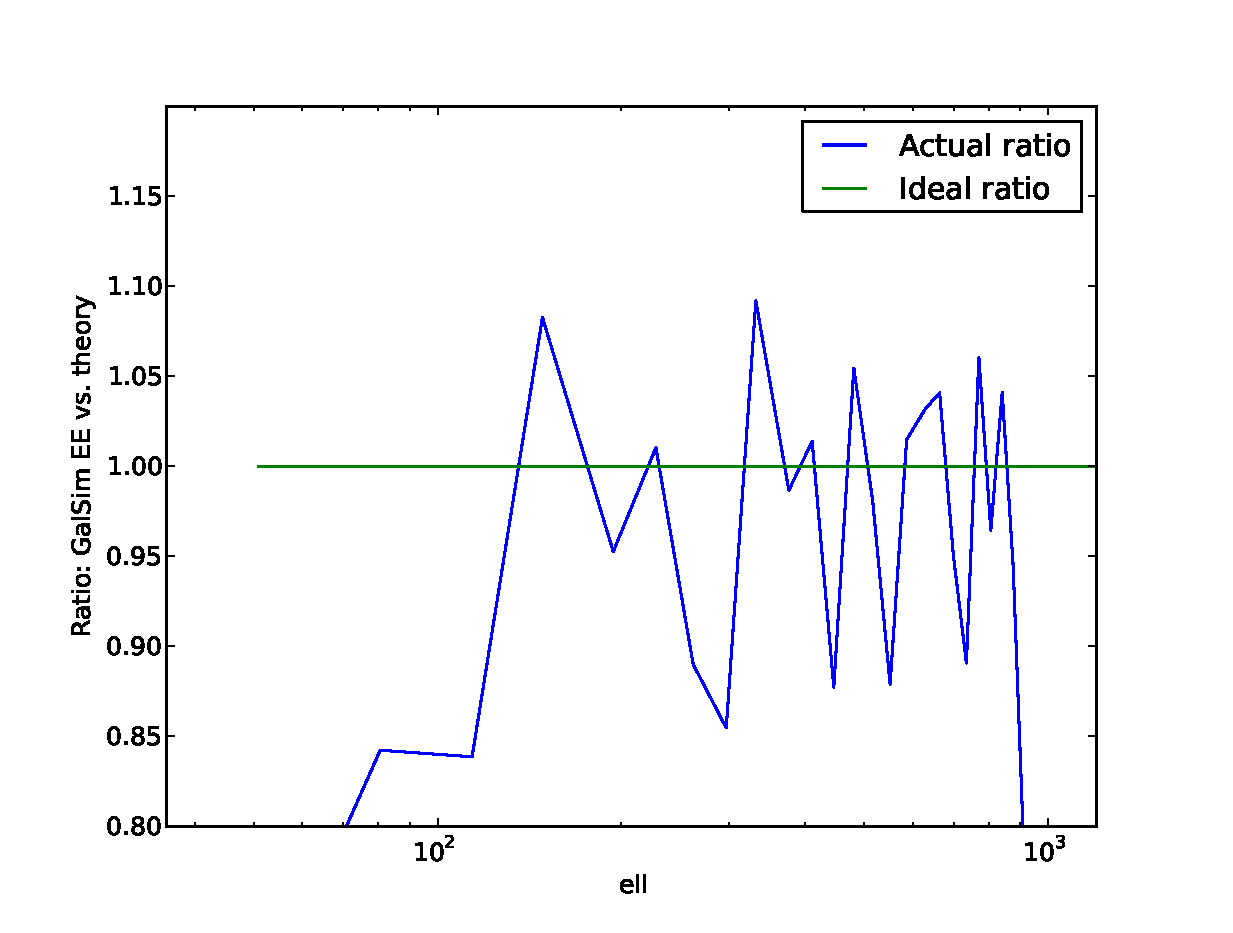
\includegraphics[width=3in]{../external/test_gridshear/output/compare_input_pe.fine.ratio.eps}
\caption{Ratio of GalSim EE PS vs. theory from Fig.~\ref{F:pe-fine}.\label{F:pe-fine-ratio}}
\end{center}
\end{figure}

We have confirmed that the results are fairly robust to the grid
spacing, for example by making the grid a factor of two more finely
spaced (and extending the WMAP7 $P(k)$ as a constant above $\ell=2000$
so that we can do this) and confirming that the results agree with
Fig.~\ref{F:pe}.

A final comment about noise: shape noise and the effect of pixel noise
in galaxy shape measurements add a term to the power, however here we
are doing tests of just the cosmological shear without either of the
above effect, so that is why it is not included in the above
formalism.  A realistic test of power spectra from simulated images
would have to include these effects.

The deficit in power at low $\ell$ is likely the same phenomenon  seem
in the CMB: the assumption of Gaussian distributions for $C_\ell$
stops being true because there aren't enough samples for the central
limit theorem to apply.  As a result, using the RMS $a_{\ell m}$ as
the inputs to the shear generation code (which is what we are
effectively doing) starts to be wrong.

\section{Shear power on larger scales than our grid}\label{S:pk0}

It is not clear that we should really be enforcing $P(k=0)=0$, i.e., no
power below our \kmin.  This is a valid condition for the full-sky
power spectrum, but will not in general be valid for a small patch of
the sky, due to cosmic variance.  In order to include this sampling
variance, it would be preferable to assign $P(k=0)$ to be some kind of
integral over $P(k<\kmin)$ (perhaps an average power in that $k$
range; details to be worked out later), {\em if} the power function is
defined for those value of $k$.  However, this limitation is only a
problem if we are checking quantities like the shear correlation
function or its value at $\theta=0$, i.e., the shear variance.  If we
are testing the ability to recover a power spectrum $P(k)$ defined at
the values of $k$ that are accessible to our grid, the $P(0)=0$
condition that we have imposed should be irrelevant.

Nonetheless, we may wish to modify the lensing engine to check whether
the power function is defined for $0< k\le\kmin$, and assign some
appropriately-weighted integral over that range as $P(k=0)$.

\end{document}
